\let\negmedspace\undefined
\let\negthickspace\undefined
\documentclass[journal]{IEEEtran}
\usepackage[a5paper, margin=10mm, onecolumn]{geometry}
%\usepackage{lmodern} % Ensure lmodern is loaded for pdflatex
\usepackage{tfrupee} % Include tfrupee package

\setlength{\headheight}{1cm} % Set the height of the header box
\setlength{\headsep}{0mm}     % Set the distance between the header box and the top of the text

\usepackage{gvv-book}
\usepackage{gvv}
\usepackage{cite}
\usepackage{amsmath,amssymb,amsfonts,amsthm}
\usepackage{algorithmic}
\usepackage{graphicx}
\usepackage{textcomp}
\usepackage{xcolor}
\usepackage{txfonts}
\usepackage{listings}
\usepackage{enumitem}
\usepackage{mathtools}
\usepackage{gensymb}
\usepackage{comment}
\usepackage[breaklinks=true]{hyperref}
\usepackage{tkz-euclide} 
\usepackage{listings}
% \usepackage{gvv}                                        
\def\inputGnumericTable{}                                 
\usepackage[latin1]{inputenc}                                
\usepackage{color}                                            
\usepackage{array}                                            
\usepackage{longtable}                                       
\usepackage{calc}                                             
\usepackage{multirow}                                         
\usepackage{hhline}                                           
\usepackage{ifthen}                                           
\usepackage{lscape}
\begin{document}
	
	\bibliographystyle{IEEEtran}
	\vspace{3cm}
	
	\title{9.9.3.17}
	\author{EE24BTECH11059 - Yellanki Siddhanth
	}
	% \maketitle
	% \newpage
	% \bigskip
	{\let\newpage\relax\maketitle}
	
	\renewcommand{\thefigure}{\theenumi}
	\renewcommand{\thetable}{\theenumi}
	\setlength{\intextsep}{10pt} % Space between text and floats
	
	
	\numberwithin{equation}{enumi}
	\numberwithin{figure}{enumi}
	\renewcommand{\thetable}{\theenumi}
	
\textbf{Question: }\\
Using integration, find the area of the region enclosed by the line $y=\sqrt{3} x$ and semi-circle $y= \sqrt{4-x^2}$ and $x$-axis in the first quadrant \\ 
\textbf{Solution: } \\
\begin{table}[h!]    
	\centering
	

	\caption{}
\end{table}\\
Line equation of form $\vec{x}=\vec{h}+k\vec{m}$
\begin{align}
	\vec{x}=\myvec{0\\0}+k\myvec{1\\ \sqrt{3}}
\end{align}
Equation of circle of form $\vec{x}^{\top}\vec{V}\vec{x}+2\vec{u}^{\top}\vec{x}+f=0$ is
\begin{align}
	\vec{u}=\myvec{0\\0},f=-4,\vec{V}=\myvec{1&0\\0&1}
\end{align}
If a line intersects the conic, $k$ value of intersecting point is given by,
\begin{align}
	k_i=\frac{-\vec{m}^{\top}\brak{\vec{Vh}+\vec{u}}\pm\sqrt{\sbrak{\vec{m}^{\top}\brak{\vec{Vh}+\vec{u}}}^2-g\brak{h}\brak{\vec{m}^{\top}\vec{Vm}}}}{\vec{m}^{\top}\vec{Vm}}
\end{align}
On substituting values of $\vec{u},\vec{m},\vec{h},\vec{V}$ we get,
\begin{align}
	k = \pm 1 
\end{align}
Since we are considering the area only in first quadrant, we will only consider $k = +1$.\\
Thus point of intersection of line with circle is $\myvec{1\\ \sqrt{3}}$.\\ 
Area bound between the semi-circle and the line is,

\begin{align}
	\vec{S} = \int_{0}^{1} x dx + \int_{1}^{2} \sqrt{4-x^{2}} dx \\
	=  \frac{1}{2} + \frac{2\pi}{3}  - \frac{1}{2} = \frac{2\pi}{3}
\end{align}
Thus area between the line and the semi-circle  is $S= \frac{2\pi}{3}$\\
	\begin{figure}[h!]
		\centering
		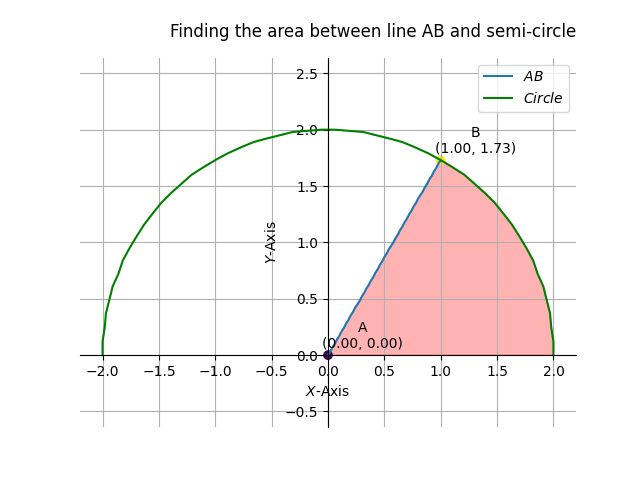
\includegraphics[width=0.9\linewidth]{figs/fig1.png}
	\end{figure}	
\end{document}  







